\documentclass{beamer}
%\usepackage{xcolor}
%\usepackage{beamerthemesplit}
\usepackage{amscd}
\usepackage{graphicx}
%\usepackage{pgf}


%\usetheme[headhight=10, footheight=10]{}
%gets rid of bottom navigation bars
\setbeamertemplate{footline}{}

%gets rid of navigation symbols
\setbeamertemplate{navigation symbols}{}

\definecolor{olive}{rgb}{0.3, 0.4, .1}
\definecolor{fore}{RGB}{249,242,215}
\definecolor{back}{RGB}{51,51,51}
\definecolor{title}{RGB}{255,0,90}
\definecolor{dgreen}{rgb}{0.,0.6,0.}
\definecolor{gold}{rgb}{1.,0.84,0.}
\definecolor{JungleGreen}{cmyk}{0.99,0,0.52,0}
\definecolor{BlueGreen}{cmyk}{0.85,0,0.33,0}
\definecolor{RawSienna}{cmyk}{0,0.72,1,0.45}
\definecolor{Magenta}{cmyk}{0,1,0,0}

\def\Z{\mathbb{Z}}
\def\R{\mathbb{R}}
\def\Q{\mathbb{Q}}
\def\H{\mathbb{H}}
\def\E{\mathbb{E}}
\def\N{\mathbb{N}}
\def\PC{{\mathbb{P}C}}
\def\CP{\mathbb{CP}}
\def\C{\mathbb{C}}
\def\L{\mathcal{L}}
\def\PSL{\textnormal{PSL}}
\def\1{\boldsymbol{1}}
\newtheorem{proposition}{Proposition}
\newtheorem{question}{Question}
\newtheorem{answer}{Answer}
\newtheorem{conjecture}{Conjecture}

\title{Kleinian groups and 3-Manifolds}
\author{Danny Calegari}
\date{February 28 2014}

\begin{document}

\frame{\titlepage}
\frame
{
\frametitle{1. Kleinian groups}

A \textcolor{blue}{Kleinian group} is a \textcolor{red}{finitely generated} and 
\textcolor{red}{discrete} group of \textcolor{red}{conformal} symmetries of the 
\textcolor{green}{sphere}, where

\begin{enumerate}
\item{``the \textcolor{green}{sphere}'' means the round unit sphere in Euclidean 3-space; and}
\item{``\textcolor{red}{conformal}'' means smooth maps which preserve angles.}
\end{enumerate}

The collection of all conformal symmetries of the sphere is a \textcolor{blue}{Lie group}; ``\textcolor{red}{discrete}''
means discrete as a subset of this group.
}
\frame
{
\begin{columns}[c]
\column{1in}
A finite group of
rotations is a Kleinian group.
\column{2in}
\begin{center}
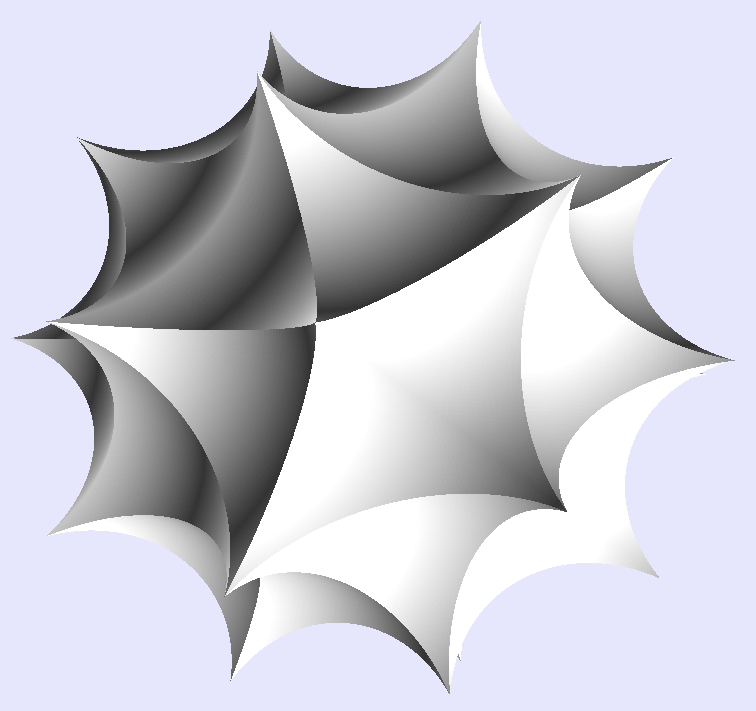
\includegraphics[width=2in]{icosahedron.png}
\end{center}
\end{columns}
}
\frame
{
\begin{columns}[c]
\column{1.1in}
The symmetries of a 
Euclidean tessellation
is a Kleinian group
by stereographic
projection.
\column{2in}
\begin{center}
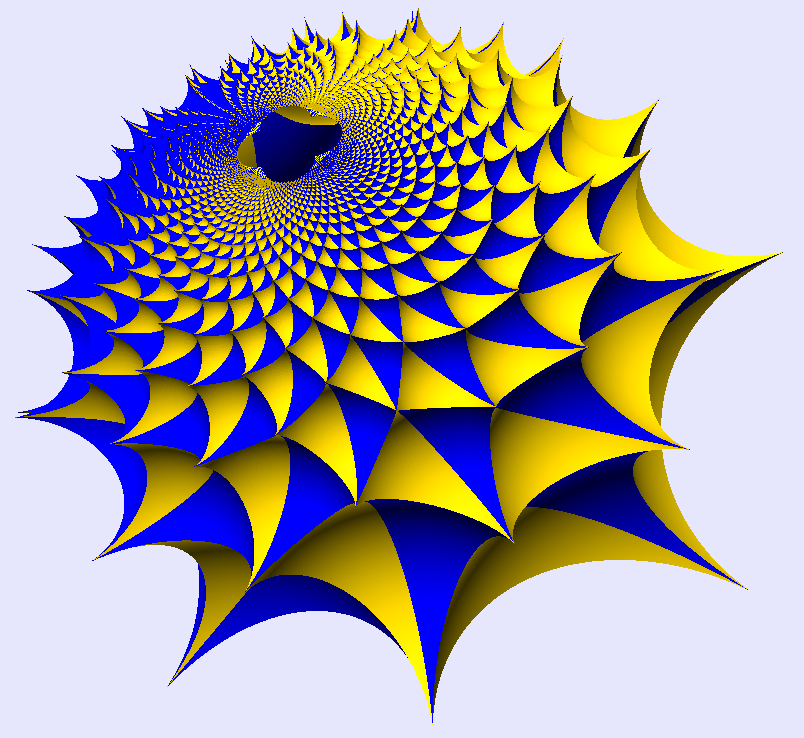
\includegraphics[width=2in]{parabolic.png}
\end{center}
\end{columns}
}
\frame
{
\begin{block}{References}
\begin{itemize}
\item{M. Bj\"orklund and T. Hartnick, {\em Biharmonic functions on groups 
and limit theorems for quasimorphisms along random walks}.
Geom. Topol. {\bf 15} (2011), no. 1, 123--143}
\item{D. Calegari and J. Maher, {\em Statistics and compression of scl}.
preprint, arXiv:1008.4952}
\end{itemize}
\end{block}
}

\end{document}

